\section{Proces}
Udviklingsprocessen er blevet udført agilt ved hjælp af sprints. Vi har i alt kørt 12 sprints, på hver én uge. I starten af processen, lå fokus meget på at designe og diskutere appen, for at gennemtænke alle features og designvalg på forhånd samt skrive det ned. Det sikrer, at appen holder sin røde tråd, selvom der er flere til at udarbejde den. Denne del resulterede i sketches (bilag \ref{sketches}) og wireframes (bilag \ref{wireframes}), og en styleguide bestående af skrifttyper, størrelser på tekst og afstande samt farveskemaer (bilag \ref{styleguide}).

Starten på vores udviklingsproces tog udgangspunkt i SCRUM, dog uden de fleste ceremonier, da vi ikke havde en product owner og scrum master. Undervejs fandt vi ud af, at mange af de ting, vi gjorde, var overdrevne, når vi kun var to, som sad fysisk sammen langt det meste af tiden. Der var for mange små detaljer, der hele tiden skulle udfyldes på trods af vores gode kommunikation. Vi besluttede derfor, at vi ikke behøvede at:

\begin{itemize}
   \item Skrive dagsorden hver gang, vi havde en arbejdsdag
   \item Skrive dybdegående user stories for hver item i vores backlog --- en to-do liste var tit nok, og i enkelte tilfælde, havde vi kun brug for en titel
   \item Sætte mærker som ``Code'' eller ``Documentation'' på små opgaver
    \item Udføre retrospectives
    \item Holde daily scrums
\end{itemize}

Med ceremonierne og mange af de formelle opgaver ude af vores arbejdsgang, vil vi ikke karakterisere processen som at være SCRUM.
Vores arbejdsgang blev derfor meget mere simpel, og vi kunne fokusere på at lave de arbejdsopgaver, som gav fremdrift i projektet, frem for at skulle holde ceremonier for at vise, hvad vi hver især havde lavet dagen forinden og i løbet af ugen. 

Processen forblev dog stadig meget struktureret, da vi holdt fast i sprints på en uge, samt at vi gjorde brug af en product- og sprint-backlog, til alle de arbejdsopgaver, som skulle udføres. 

Efter hver arbejdsopgave sørgede vi for at holde det, vi havde lavet, op imod vores \textit{Definition of Done}. Det gjorde, at vi f.eks. altid var sikre på, at den kode, som vi lagde på vores master branch, compilede, samt at vores unit- og instrumentation-tests altid var succesfulde.

Vi fortsatte ydermere med at lave estimeringer og give hver opgave et antal story points, så vi kunne holde styr på hvor meget vi manglede, og hvilke opgaver, der var store og små. Disse estimeringer blev også brugt til at give os et overblik, da de blev visualiseret i form af et burn-up chart.

\subsection{Burn-up chart}
Vi har undervejs i projektet gjort brug af et burn-up chart for at se udviklingen i projektet. Lige inden start på et nyt sprint, opdaterede vi vores graf. Det gav os et overblik over hvor meget, vi var nødt til at tage med i hvert sprint, for at kunne blive færdige til tiden. Det, at vi har visualiseret vores story points og ikke udelukkende regnet på formlen \medskip

\textit{story points = (total story points - færdige points) / antal sprints tilbage} \smallskip

gav os et ekstra overblik. Vi kunne således se hvordan vores backlog havde ændret sig i løbet af de forrige sprints samt hvordan vores sprint backlog havde justeret sig.  Vi sørgede så for altid at tage flere point med i sprintet end der var nødvendigt, da vi næsten altid fik flere opgaver ind efter et sprint var slut. Disse opgaver kom typisk fra en brugertest, men kunne også være som følge af problemer eller idéer, som vi selv kom frem til.

\begin{figure}[H]
    \centering
    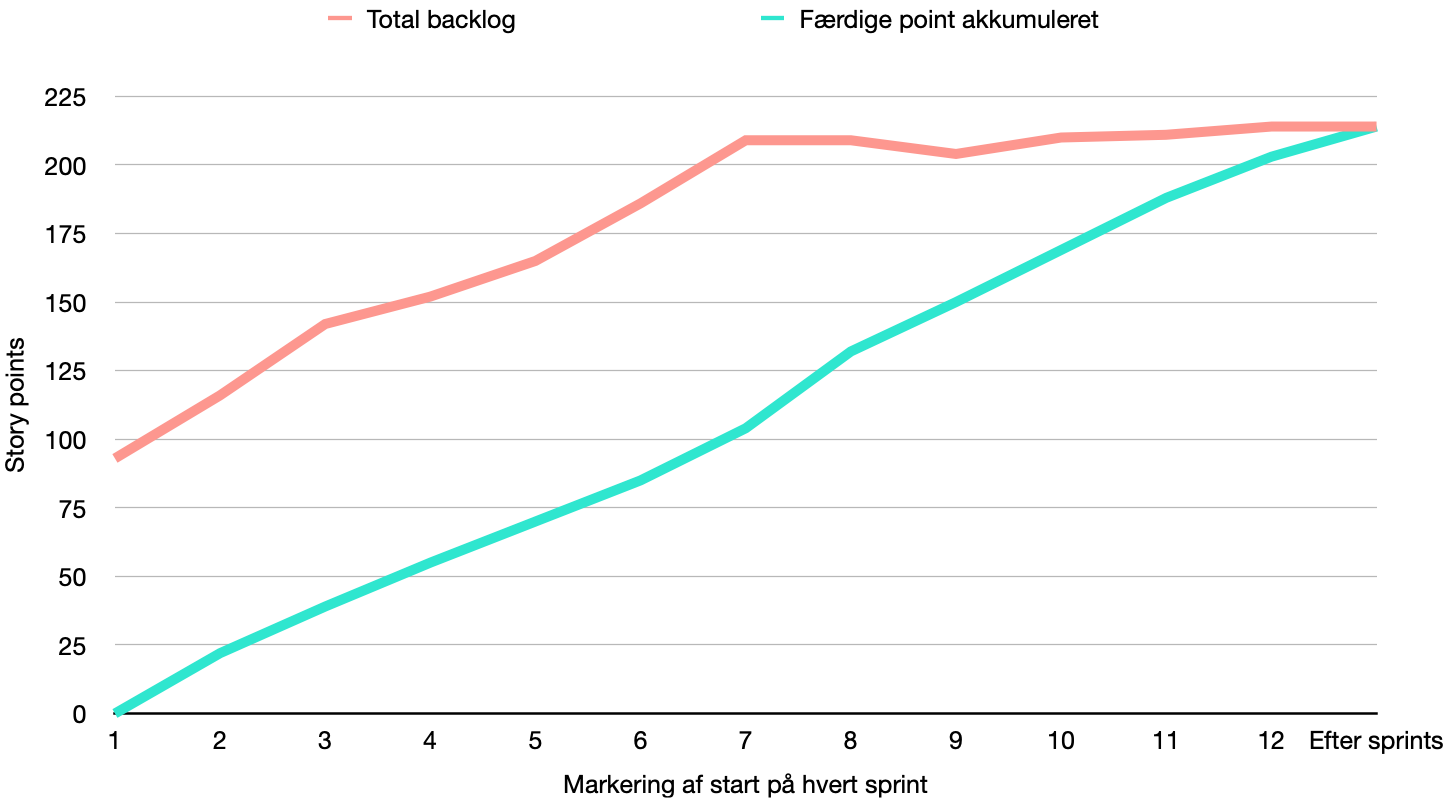
\includegraphics[width=1\textwidth]{img/burn-up-chart.png}
    \caption{Burn-up chart}
    \label{burn-up}
\end{figure}

Fordelen ved at bruge et burn-up chart frem for burn-down er, at man kan se hvordan backloggen ændrer sig. I et burn-down chart er der kun de resterende point visualiseret. To sprints med samme deltaværdi kan dermed have haft vidt forskellige ændringer i den totale backlog og sprint backloggen. Ved at bruge et burn-up chart er det nemmere at tage højde for, at backloggen ændrer sig i løbet af projektet.
